\documentclass[12pt,a4paper]{article}

% ============================================================
% Packages
% ============================================================
\usepackage[utf8]{inputenc}
\usepackage[T1]{fontenc}
\usepackage{lmodern}
\usepackage[english]{babel}
\usepackage{csquotes}
\usepackage{amsmath,amssymb}
\usepackage{booktabs}
\usepackage{tabularx}
\usepackage{adjustbox}
\usepackage{graphicx}
\usepackage{xcolor}
\usepackage[hypertexnames=false]{hyperref}
\usepackage{cleveref}
\usepackage{float}

% APA citations via biblatex
\usepackage[style=apa,backend=biber,natbib=true]{biblatex}
\addbibresource{references.bib}
\DeclareLanguageMapping{english}{english-apa}

% ============================================================
% Custom commands
% ============================================================
\newcommand{\xscore}{\textit{xScore}}
\newcommand{\xvoa}{\textit{xVOA}}
\newcommand{\gds}{\textit{GDS}}

% Formatting
\emergencystretch=2em
\widowpenalty=10000
\clubpenalty=10000

\title{Game Deserved Score: Decomposing NFL Team Quality\\and Testing the Defensive Dominance Hypothesis}
\author{Lasse Mecha}
\date{2026}

\begin{document}
\maketitle

% ============================================================
% ABSTRACT
% ============================================================
\begin{abstract}
We introduce the Game Deserved Score (\gds{}), a fully transparent, reproducible framework that decomposes NFL team quality into three additive components -- offensive, defensive, and special teams expected value over average (\xvoa{}) -- built on drive-level expected-point predictions from a calibrated multinomial model (\xscore{}; \citealt{mecha2026xscore-model}). Across 2,119 regular-season games (2018--2025), the team with higher \gds{} wins 85.7\% of contests, and mean \gds{}/game explains 74.3\% of season win-percentage variance ($r = 0.862$, $n = 256$ team-seasons). We then use \gds{} to conduct the first systematic, multi-method test of the widely cited claim that ``defense wins championships.'' Decomposing team quality into offensive and defensive \xvoa{}, we classify all 256 team-seasons by archetype dominance and test three directional hypotheses via five statistical procedures: Spearman rank correlation, Pearson correlation with $R^2$ decomposition, binary logistic regression, OLS regression, and Cohen's $d$ effect size estimation. All three hypotheses are rejected. Offensive \xvoa{} explains 2.6 times more win-percentage variance than defensive \xvoa{} (44.5\% vs.\ 16.9\%), offense-dominant teams dramatically outperform defense-dominant teams in playoff advancement (Cohen's $d = 0.669$, 95\% CI $[0.580, 0.776]$), and every one of the eight Super Bowl champions in the study window was offense-dominant. Not a single defense-dominant team-season -- 32 of them across eight seasons -- won more than one playoff game. Because the sample extends through the 2025 season, 32 of the 256 team-seasons -- one full season -- and one of the eight championships were entirely unseen when the underlying measurement framework was first developed; the qualitative pattern holds unchanged on this genuinely out-of-sample data, while the point estimate of the offense-to-defense ratio attenuates from an earlier 3.3:1 (2018--2024 only) to 2.6:1 -- a more conservative estimate that we report as evidence of the finding's stability rather than suppress in favor of the larger number. Robustness checks -- opponent-strength control, field-position mediation, and sensitivity to both the archetype threshold and the time window -- confirm the offensive advantage never drops below 2.5:1 in any subwindow tested. These are correlational, not causal, findings: any resource-allocation implications are conditional on the observed associations partially reflecting causal mechanisms, a qualification we carry through the abstract, introduction, and discussion rather than confining to a caveat late in the paper. \gds{} and the complete analytical pipeline are open-source and publicly available.
\end{abstract}

\textbf{Keywords:} team quality measurement, expected points, NFL analytics, performance decomposition, defense wins championships, playoff prediction

% ============================================================
% 1. INTRODUCTION
% ============================================================
\section{Introduction}
\label{sec:introduction}

Each of the NFL's 32 franchises operates under a hard salary cap -- \$301.2 million per team for 2026 \citep{nfl2026cap} -- that imposes a strict zero-sum constraint on roster construction \citep{nflcba2020}. The cap does not distinguish offensive from defensive spending; it is a single ceiling on total player cost. Every allocation decision is therefore implicitly a trade-off, and at a combined annual expenditure approaching \$10 billion across all clubs, even a modest misallocation driven by a faulty heuristic represents cumulative opportunity cost in the hundreds of millions per year.

For decades the dominant heuristic guiding this allocation has been a single phrase, popularly attributed to Alabama coach Paul ``Bear'' Bryant: ``offense wins games, defense wins championships'' \citep{williams2010bearbryant}. It is a specific, testable empirical claim -- that defensive quality becomes decisive in the postseason even where offensive quality drives regular-season success -- and it pervades coaching philosophy, media narrative, and player discourse. Yet the NFL's competitive environment has shifted substantially since the phrase entered common use: beginning with the 2004 restrictions on downfield contact \citep{nflops2004rules} and continuing through expanded roughing-the-passer enforcement \citep{pereira2018roughing}, the league has systematically tilted the rules toward passing offenses, and the 2020s have produced the highest-scoring seasons in NFL history \citep{barnwell2019passingrevolution, nflscoring2023trends}. Whether a defense-first heuristic formed in a lower-scoring era still holds is an empirical question, not a matter of tradition.

Testing it rigorously requires a measurement instrument that existing metrics do not provide. Expected Points Added (EPA) offers a common currency for play evaluation but aggregates noisily to the team level and does not decompose into offensive and defensive contributions \citep{carl2021nflfastr}. Defense-adjusted Value Over Average (DVOA) does decompose team quality by phase, but its opponent-adjustment algorithm has never been published, and no external researcher has replicated its figures \citep{schatz2005dvoa}. Pro Football Focus grades rely on subjective analyst judgment that is inherently non-reproducible. \citet{robst2011defense} published the only prior peer-reviewed test of the defensive hypothesis, using aggregate box-score statistics from 1981--2009 and finding offense the stronger predictor of Super Bowl success -- but their independent variables conflate quality with game-script opportunity (a team protecting a large lead allows garbage-time yards that inflate opponent statistics without reflecting genuine defensive weakness), and no subsequent peer-reviewed study has revisited the question with modern data or methods.

We address this gap in two steps. First, we introduce the Game Deserved Score (\gds{}), a fully transparent, reproducible framework decomposing NFL team quality into three additive components -- offensive expected value over average (Off\_\xvoa{}), defensive expected value over average (Def\_\xvoa{}), and special teams value (ST\_Value) -- built on drive-level expected-point predictions from a calibrated multinomial model (\xscore{}; \citealt{mecha2026xscore-model}) and expressed on a common expected-points scale. Across 2,119 regular-season games (2018--2025), the team with higher \gds{} wins 85.7\% of contests, and mean \gds{}/game explains 74.3\% of season win-percentage variance ($r=0.862$, $n=256$ team-seasons) -- establishing \gds{} as a validated measure of deserved competitive performance before we use it for anything else. Second, we apply the validated framework to the championship hypothesis directly, decomposing team quality into offensive and defensive \xvoa{} and testing three directional hypotheses operationalizing the defensive claim:

\begin{description}
  \item[H1 (Postseason advancement).] Defense-dominant team-seasons (offense share $< -0.3$) achieve higher mean playoff-win totals than offense-dominant team-seasons (offense share $> +0.3$).
  \item[H2 (Super Bowl over-representation).] Super Bowl winners are disproportionately drawn from defense-dominant team-seasons relative to the base rate of defense dominance among all playoff qualifiers.
  \item[H3 (Correlation asymmetry).] Defensive \xvoa{} per game exhibits a stronger monotonic association with playoff wins among playoff teams than offensive \xvoa{} per game does.
\end{description}

Each hypothesis is stated so that support would be consistent with the defensive narrative; the three are logically independent, so convergent rejection is not an artifact of any single operationalization. We test all three via five statistical procedures with different assumptions and sensitivities -- Spearman rank correlation, Pearson correlation with $R^2$ decomposition, binary logistic regression, OLS regression, and Cohen's $d$ -- and find all three rejected, convergently, across every procedure. We state directly here, rather than only in the Discussion, that these are correlational findings: the analysis documents statistical association between team quality components and competitive outcomes, not a demonstration that investing in offense causes teams to win. Any resource-allocation implications we draw are conditional on these associations partially reflecting causal mechanisms.

The sample spans eight complete NFL seasons (2018--2025). This is a deliberate design choice rather than an incidental one: the underlying \xscore{} model was trained on 2018--2024 data with 2025 held out as a genuine test set \citep{mecha2026xscore}, so applying it to compute team quality for the 2025 season -- including that season's Super Bowl champion -- provides an out-of-sample check on every finding in this paper, not merely a larger version of the same analysis. We report where the pattern holds unchanged on this new data and where the point estimates move, rather than reporting only the version of the analysis that produces the largest effect.

This paper makes three contributions. First, it provides the first fully open-source, reproducible team-quality metric with an explicit three-component decomposition, validated against actual game outcomes before being applied to any downstream question. Second, it provides the first multi-method test of the defensive championship hypothesis using calibrated drive-level measurement rather than aggregate box-score statistics, extending \citet{robst2011defense} to the modern rule era and validating the result on data the measurement framework had not seen when it was built. Third, it introduces the ``competent defense threshold'' as a theoretical framework moving beyond binary offense-versus-defense framing: offensive quality is the primary engine of playoff advancement, while defensive adequacy operates as a necessary but insufficient secondary condition. The remainder of the paper describes the data and probability baseline, the \gds{} framework and its validation, the archetype classification methods, the hypothesis-testing results and robustness checks, and the strategic and theoretical implications.

% ============================================================
% 2. RELATED WORK
% ============================================================
\section{Related Work}
\label{sec:related-work}

\subsection{Existing Team-Quality Metrics}
\label{sec:existing-metrics}

Three families of metrics attempt to measure team quality, and none provides a transparent, reproducible three-component decomposition. EPA assigns a point value to every game state and measures the change each play creates, providing a common currency for play comparison \citep{carter1971operations, carl2021nflfastr}. It is well suited to within-game play evaluation but, aggregated to the team level, suffers from play-level noise (single explosive plays dominate season totals), within-drive attribution problems (cooperative sequences treated as independent value-creating events), and game-script compression (leading teams' EPA suppressed by conservative play-calling). DVOA decomposes performance into offensive, defensive, and special-teams components and adjusts for opponent quality, but the adjustment algorithm, weighting function, and normalization procedure have never been published \citep{schatz2005dvoa}; no external researcher has independently replicated its figures, and claims about which teams have the best defense rest on authority rather than verifiable methodology. Pro Football Focus grades every player on every play, but grading is inherently non-reproducible across analysts and the play-to-season weighting scheme is proprietary \citep{pff2014grades}. Win probability models \citep{stern1991probability, lock2014randomforests} share \xscore{}'s commitment to situational conditioning but predict the binary game outcome rather than the multinomial drive outcome, and so cannot attribute value to offense, defense, or special teams separately.

No existing approach provides all four properties simultaneously: a calibrated probability baseline independent of team identity, an explicit three-component decomposition, a common expected-point scale enabling direct comparison across components, and a fully open-source implementation enabling independent replication. EPA satisfies the fourth property but not the first three; DVOA satisfies the second and third but not the first or fourth; PFF satisfies none. \gds{} is designed to satisfy all four, and does so by extending Expected Possession Value-style decomposition \citep{cervone2016multiresolution} to the drive level: rather than asking which team scored more, it asks which team generated and suppressed scoring probability at a rate inconsistent with league expectations, and by how much. \gds{} achieves comparable discriminative validity to publicly reported DVOA win-percentage correlations ($r \approx 0.85$) while being fully reproducible -- the advantage is not merely decomposition but a \emph{calibrated} drive-level baseline, since \xscore{}'s verified Expected Calibration Error of 0.010 ensures the denominators in the \xvoa{} calculation match observed frequencies, a property no existing public metric has demonstrated. The trade-off is that \gds{} does not adjust for opponent quality at the drive level as DVOA claims to, relying instead on large-sample averaging across a full season to attenuate schedule effects; \Cref{sec:robustness-design} reports an explicit test of whether this matters for the paper's conclusions.

\subsection{The ``Defense Wins Championships'' Debate}
\label{sec:dwc-debate}

\citet{robst2011defense} published the only direct peer-reviewed examination of the defensive hypothesis. Using data from 1981 through 2009, they employed logistic regression to predict Super Bowl participation and victory from total offensive yards, total defensive yards allowed, points scored, points allowed, turnover differential, and strength of schedule, finding offensive metrics -- particularly points scored and offensive yards -- substantially stronger predictors than defensive metrics. Their directional conclusion is consistent with the present study, but their independent variables are aggregate box-score statistics that conflate quality with game-script opportunity: a team protecting a large lead allows yards and points in garbage time that inflate its defensive statistics without reflecting genuine weakness, while a team trailing accumulates passing yards against prevent defenses. No machine learning, game-state conditioning, or drive-level granularity was available to them, and their sample predates the modern passing revolution. No subsequent peer-reviewed study has revisited the hypothesis with modern data or methods in the fifteen years since. \citet{lock2014randomforests} independently found offensive variables consistently more predictive of NFL game outcomes than defensive variables using random forests at the game level -- a different methodological tradition reaching the same directional conclusion, which strengthens confidence that the finding is not an artifact of any single analytic framework.

Any investigation of championship predictors must also contend with the dominant role of randomness in single-elimination playoffs: a team plays at most four postseason games en route to a title, so a single turnover, injury, or officiating decision can end a season regardless of underlying quality \citep{lopez2018randomness}. This motivates multi-season aggregation and convergence across multiple statistical procedures rather than reliance on any single test.

\subsection{Resource Allocation Under Salary Cap Constraints}
\label{sec:resource-allocation-lit}

The NFL's hard salary cap creates a zero-sum dynamic largely absent from leagues with soft caps or uncapped spending \citep{lewis2003moneyball}: every team has the same budget, and the only variable is how it is allocated. \citet{mulholland2019optimizing} modeled the marginal win-value of salary-cap spending at each position group and found quarterback spending the single most efficient allocation, consistent with offensive quality driving winning, with the gap between current league-average allocation and theoretically optimal allocation substantial. \citet{massey2013loserscurse} demonstrated that NFL teams systematically overvalue early draft picks relative to the surplus production those picks generate -- a market inefficiency that compounds any allocation problem: if a defense-first heuristic drives teams to deploy premium draft capital on defensive positions while offensive investment in fact delivers superior returns, the resulting misallocation uses the most overpriced acquisition mechanism available on the wrong side of the ball.

% ============================================================
% 3. DATA, XSCORE RECAP, AND THE GDS FRAMEWORK
% ============================================================
\section{Data, \xscore{} Recap, and the \gds{} Framework}
\label{sec:framework}

\subsection{Data Source and Scope}
\label{sec:data}

All data are sourced from \texttt{nflfastR} \citep{carl2021nflfastr} via the Python \texttt{nfl\_data\_py} wrapper \citep{cooper2023nfldatapy}. The \xscore{} model (\Cref{sec:xscore-recap}) is trained on 241,195 filtered plays across 41,117 drives from seven NFL seasons (2018--2024) and evaluated on a held-out 2025 test set (34,415 plays across 5,803 drives). The team-quality analysis in this paper -- \gds{} construction, validation, and the hypothesis tests in \Cref{sec:methods,sec:descriptive,sec:hypothesis-tests} -- uses the trained model to score all eight seasons, 2018--2025 inclusive (256 team-seasons), so the 2025 season enters every downstream result as genuinely out-of-sample data rather than as part of model training. Play filtering retains pass, rush, and sack plays and excludes kickoffs, punts, extra points, two-point conversions, kneels, spikes, and aborted snaps. The 2018 lower bound reflects the structural break in scoring distributions created by the rule changes discussed in \Cref{sec:introduction} \citep{pereira2018roughing}. A drive begins when a team takes possession and ends at a terminal event -- touchdown, field goal, turnover, punt, or end of half/game -- and is the natural unit for team quality measurement because it encompasses the full cooperative sequence of plays within a single possession. The target variable is categorical: $y \in \{\text{TD}, \text{FG}, \text{Turnover}, \text{Punt/Other}\}$.

\subsection{The \xscore{} Model}
\label{sec:xscore-recap}

The expected-points baseline is provided by \xscore{}, a calibrated multinomial XGBoost model that predicts $P(\text{TD} \mid s)$, $P(\text{FG} \mid s)$, $P(\text{TO} \mid s)$, $P(\text{Punt} \mid s)$ from seven situational features describing the game state at the drive's start: down, yards to go, field position, score differential, time remaining in half, a goal-to-go indicator, and a red zone indicator. Team identity is deliberately excluded from the feature set, producing a league-average expected-performance baseline independent of who is playing -- deviations from this baseline therefore measure team quality rather than circular self-prediction. Trained and evaluated on the data described in \Cref{sec:data}, the model achieves a multiclass Brier score of 0.1562 on the held-out 2025 test set (Brier Skill Score 15.3\% over a naive marginal-frequency baseline), with per-class AUC-ROC ranging from 0.680 (turnover) to 0.813 (punt/other). Per-class isotonic calibration ensures predicted probabilities closely match observed frequencies across the full probability range, with a mean Expected Calibration Error of 0.010. Temporal generalization to pre-rule-change seasons (2014--2017; 134,274 plays across 23,802 drives) yields an equivalent Brier score of 0.1529, confirming stability across regulatory eras. SHAP analysis confirms the model's learned feature hierarchy -- field position dominant, followed by down and distance -- matches established domain knowledge rather than an artifact of overfitting.

The four-class probability vector converts to a single expected-points figure via:
\begin{equation}
  \label{eq:xep}
  \text{xEP}(s) = 7 \cdot \hat{P}(\text{TD} \mid s)
                 + 3 \cdot \hat{P}(\text{FG} \mid s)
                 + 0 \cdot \hat{P}(\text{Punt} \mid s)
                 - \text{EP}_{\text{opp}}(yl) \cdot \hat{P}(\text{TO} \mid s),
\end{equation}
where $\text{EP}_{\text{opp}}(yl)$ is a field-position-dependent turnover penalty computed as the mean observed actual points across all training-window drives that began at the corresponding opponent yardline. \xscore{} conditions on score differential, so the baseline already accounts for game-script effects: a team protecting a large lead receives lower xEP baselines (conservative play expected), so conservative drives that produce punts generate minimal negative \xvoa{} rather than being penalized as if the team were still playing to score. This conditioning is what distinguishes the framework from raw EPA aggregation, which does not adjust for game state in the same way.

Calibration is essential to everything that follows: \gds{} treats \xscore{} outputs as genuine expected values, so any systematic miscalibration would propagate into biased team-quality estimates. We report the model's validation evidence here in enough detail that a reader can assess it directly rather than taking it on trust from an external source; full training procedure, feature engineering, hyperparameter search, and extended validation are reported in the working paper that first developed the model \citep{mecha2026xscore}, and a peer-reviewed treatment of the model specifically is a separate, standalone submission under review as this paper is written.

\subsection{The \gds{} Framework: Three-Component Decomposition}
\label{sec:gds-construction}

\gds{} decomposes game-level deserved performance into three additive channels: Off\_\xvoa{}, Def\_\xvoa{}, and ST\_Value. The decomposition is exhaustive -- every drive routes through exactly one channel. For a team $A$ in a game against opponent $B$:
\begin{equation}
  \label{eq:gds}
  \gds(A) = \xvoa{}_{\mathrm{Off}}(A) + \xvoa{}_{\mathrm{Def}}(A) + \mathrm{ST}(A).
\end{equation}
A \gds{} of $+7.0$ means the team generated one full touchdown of net positive performance beyond league-average expectations in identical circumstances. \Cref{fig:pipeline} provides a schematic overview of the computation pipeline.

\begin{figure}[htbp]
  \centering
  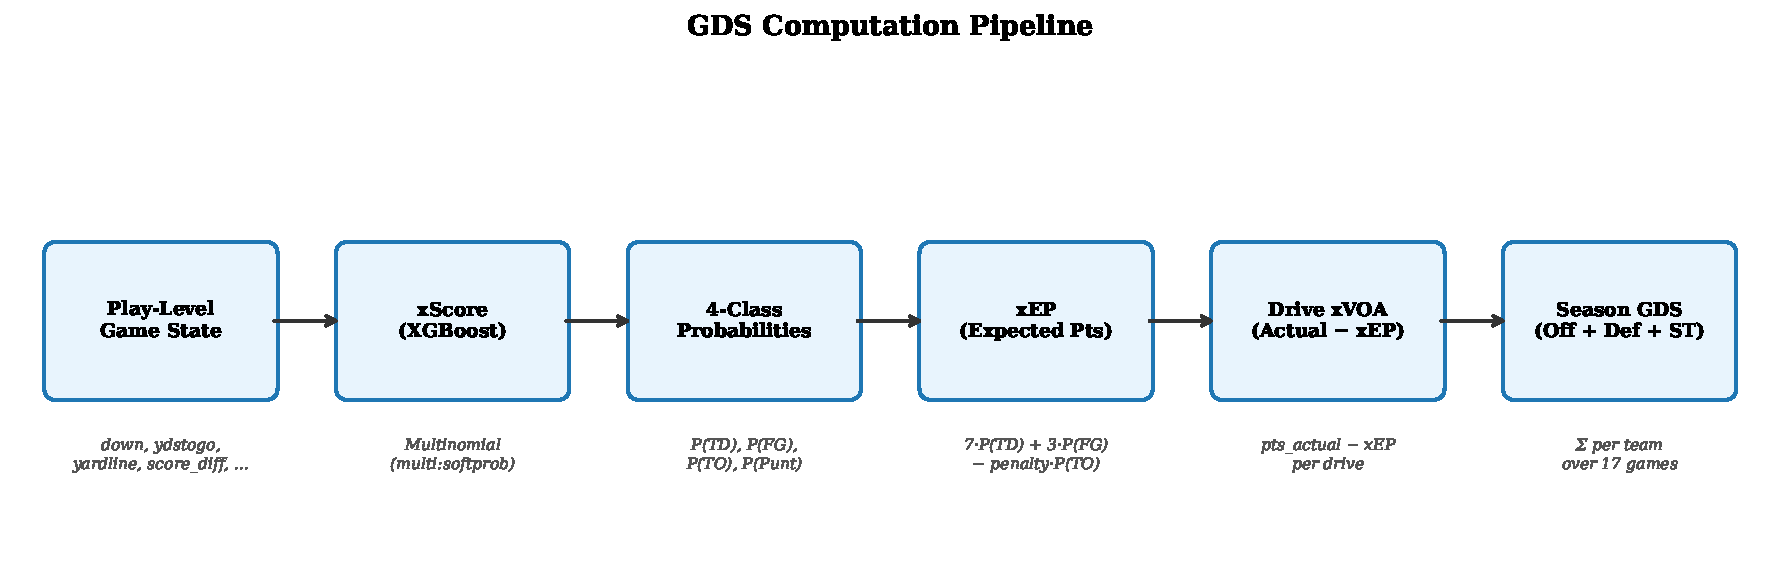
\includegraphics[width=\textwidth]{figures/fig9_pipeline_flowchart.pdf}
  \caption{End-to-end \gds{} computation pipeline. Situational game-state features feed into the multinomial \xscore{} model, producing four-class drive outcome probabilities that are converted to expected points (xEP). Drive-level value over average (\xvoa{}) is aggregated to season-level \gds{} decomposed into offensive, defensive, and special-teams contributions.}
  \label{fig:pipeline}
\end{figure}

\paragraph{Offensive \xvoa{}.} Let $\text{pts}(d)$ denote the actual points scored on drive $d$ (7 for an offensive touchdown, 3 for a made field goal, 0 otherwise). Per-drive offensive value added is:
\begin{equation}
  \label{eq:xvoa-drive}
  \xvoa{}^{(d)} = \mathrm{pts}(d) - \mathrm{xEP}\!\bigl(s_1^{(d)}\bigr),
\end{equation}
and game-level Off\_\xvoa{} sums this across all of a team's drives in a game. A drive beginning with $\text{xEP} = 2.8$ that ends in a touchdown generates $+4.2$ \xvoa{} (substantial overperformance); the same starting state ending in a punt generates $-2.8$ (failure to convert a state with meaningful scoring expectation). This graduated accounting -- distinguishing 7-point, 3-point, and 0-point outcomes against the same situational denominator -- is the primary advantage of the multinomial model over binary (touchdown vs.\ not) approaches, which collapse the FG/punt/turnover distinction entirely.

\paragraph{Defensive \xvoa{}.} No separate defensive model is required: $\xvoa{}_{\mathrm{Def}}(A) = -\,\xvoa{}_{\mathrm{Off}}(B)$. The opponent's offensive \xvoa{} measures points generated beyond situational expectation against team $A$'s defense; negating it converts this into a defensive penalty or credit. This construction guarantees Off/Def contributions sum to zero across both teams in every game, and avoids the attribution ambiguity that would arise from computing defensive \xvoa{} directly from defensive plays (sacks, deflections), which overlap with offensive drive sequences and risk double-counting.

\paragraph{Special teams value.} ST\_Value captures field-position advantage conferred at drive start relative to transition-type baselines (kickoff, punt, missed field goal, interception, fumble, downs). The expected starting xEP for each transition type $\tau$ is estimated empirically as $\mu_{\tau}$, the mean xEP at drive start across all training-window drives of that type, computed once and held fixed to prevent leakage. Per-drive ST value is the deviation from this baseline, $\mathrm{ST}^{(d)} = \mathrm{xEP}(s_1^{(d)}) - \mu_{\tau(d)}$, summed to the game level. A team with consistently good kick returns will systematically start kickoff drives above $\mu_{\texttt{KICKOFF}}$, generating positive ST\_Value.

\paragraph{Turnover attribution.} A potential concern is whether the same play could contribute to multiple components. It cannot: the turning team's offensive channel absorbs the full cost ($0 - \text{xEP}(s_1) < 0$); the receiving team's ST channel receives the field-position credit (compared to the \texttt{INT} or \texttt{FUM} baseline); and the receiving team's defensive channel receives suppression credit only through $-\text{Off\_\xvoa{}}$(turning team), with no additional entry. No play is counted in more than one channel.

\paragraph{Formal properties.} Four properties support analytical use: (1) \textbf{zero-sum} -- Off/Def contributions sum to zero across both teams in every game, so $\gds(A) + \gds(B) = \mathrm{ST}(A) + \mathrm{ST}(B)$; (2) \textbf{unified scale} -- all components are in expected-point units, so Off\_\xvoa{} of $+1.0$ represents the same advantage as ST\_Value of $+1.0$; (3) \textbf{additivity} -- game-level values sum to season totals at every aggregation level; (4) \textbf{decomposability} -- any single channel's contribution can be isolated at per-game, per-week, per-season, or subset level.

\subsection{Validation: \gds{} Predicts Winning}
\label{sec:validation}

Before using \gds{} to test anything about offense and defense, we validate that it measures genuine competitive quality across all eight seasons. Across 2,119 regular-season games (2018--2025, excluding ties), the team with higher \gds{} won 1,815 times -- \textbf{85.7\%} game-winner accuracy, a 28.7 percentage-point improvement over the 57\% home-team baseline \citep{lopez2018randomness}. This comparison is ``noiseless'' in the relevant sense: \gds{} is computed entirely from execution on the game day itself, without using final score or opponent identity as input, so the 14.3\% of games where the lower-\gds{} team won are not measurement error but games where football's structural variance -- turnover bounces, field-goal efficiency, explosive-play timing -- decoupled process from scoreboard.

At the season level ($n=256$ team-seasons), mean \gds{}/game correlates $r = 0.862$ with win percentage ($R^2 = 0.743$, $p = 6.1 \times 10^{-77}$; \Cref{fig:gds-winpct}). Component decomposition (\Cref{tab:components}) shows offensive \xvoa{} alone explains $R^2 = 44.5\%$ of win-percentage variance and defensive \xvoa{} alone explains $R^2 = 16.9\%$ -- a \textbf{2.6:1 ratio} that is the paper's central structural finding, reported once here and used in \Cref{sec:hypothesis-tests} as the primary evidence for H3. This ratio is a more conservative estimate than the 3.3:1 obtained from the original 2018--2024 sample alone; \Cref{sec:hypothesis-tests,sec:strategic} treat 2.6:1 as the paper's headline number precisely because it includes the out-of-sample 2025 season, and \Cref{tab:robustness-summary} shows the ratio never falls below 2.5:1 in any time window tested. The combined $R^2$ (74.3\%) exceeds the sum of the individual $R^2$ values (61.4\%) by 12.9 percentage points, indicating synergistic structure: teams strong on both dimensions outperform additive expectation, which is why we treat \gds{} as a unified index rather than a simple sum of independent components.

\begin{figure}[htbp]
  \centering
  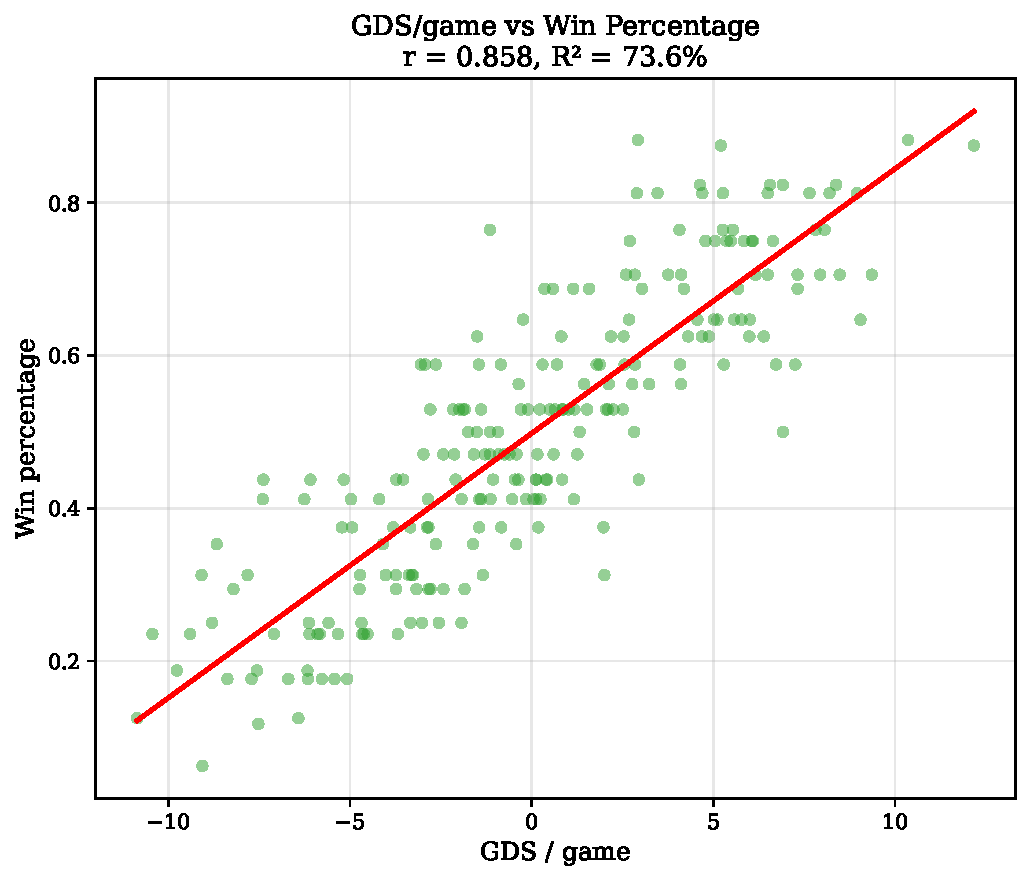
\includegraphics[width=0.75\textwidth]{figures/fig6_gds_vs_winpct.pdf}
  \caption{Season-level \gds{}/game versus win percentage ($n=256$ team-seasons, 2018--2025). The tight linear relationship ($r=0.862$, $R^2=74.3\%$) confirms that \gds{} captures the competitive quality dimension that drives winning.}
  \label{fig:gds-winpct}
\end{figure}

\begin{table}[htbp]
  \centering
  \caption{Correlation between individual \gds{} components and season win percentage ($n=256$ team-seasons, 2018--2025). This is the source table for the 2.6:1 offense-to-defense ratio referenced throughout the paper; it is not restated elsewhere.}
  \label{tab:components}
  \begin{tabular}{lcc}
    \toprule
    \textbf{Metric} & \textbf{Pearson $r$} & \textbf{$R^2$} \\
    \midrule
    Off\_\xvoa{}/game  & 0.667 & 44.5\% \\
    Def\_\xvoa{}/game  & 0.412 & 16.9\% \\
    Combined \gds{}/game & 0.862 & 74.3\% \\
    \bottomrule
  \end{tabular}
\end{table}

\Cref{fig:xvoa-winpct} visualizes the component split directly: the tighter clustering and steeper regression line for offense show the same 2.6:1 discrepancy in variance explained that \Cref{tab:components} reports numerically. \Cref{tab:top-bottom} illustrates the component structure concretely with the five highest- and lowest-\gds{} teams in the 2024 season.

\begin{figure}[htbp]
  \centering
  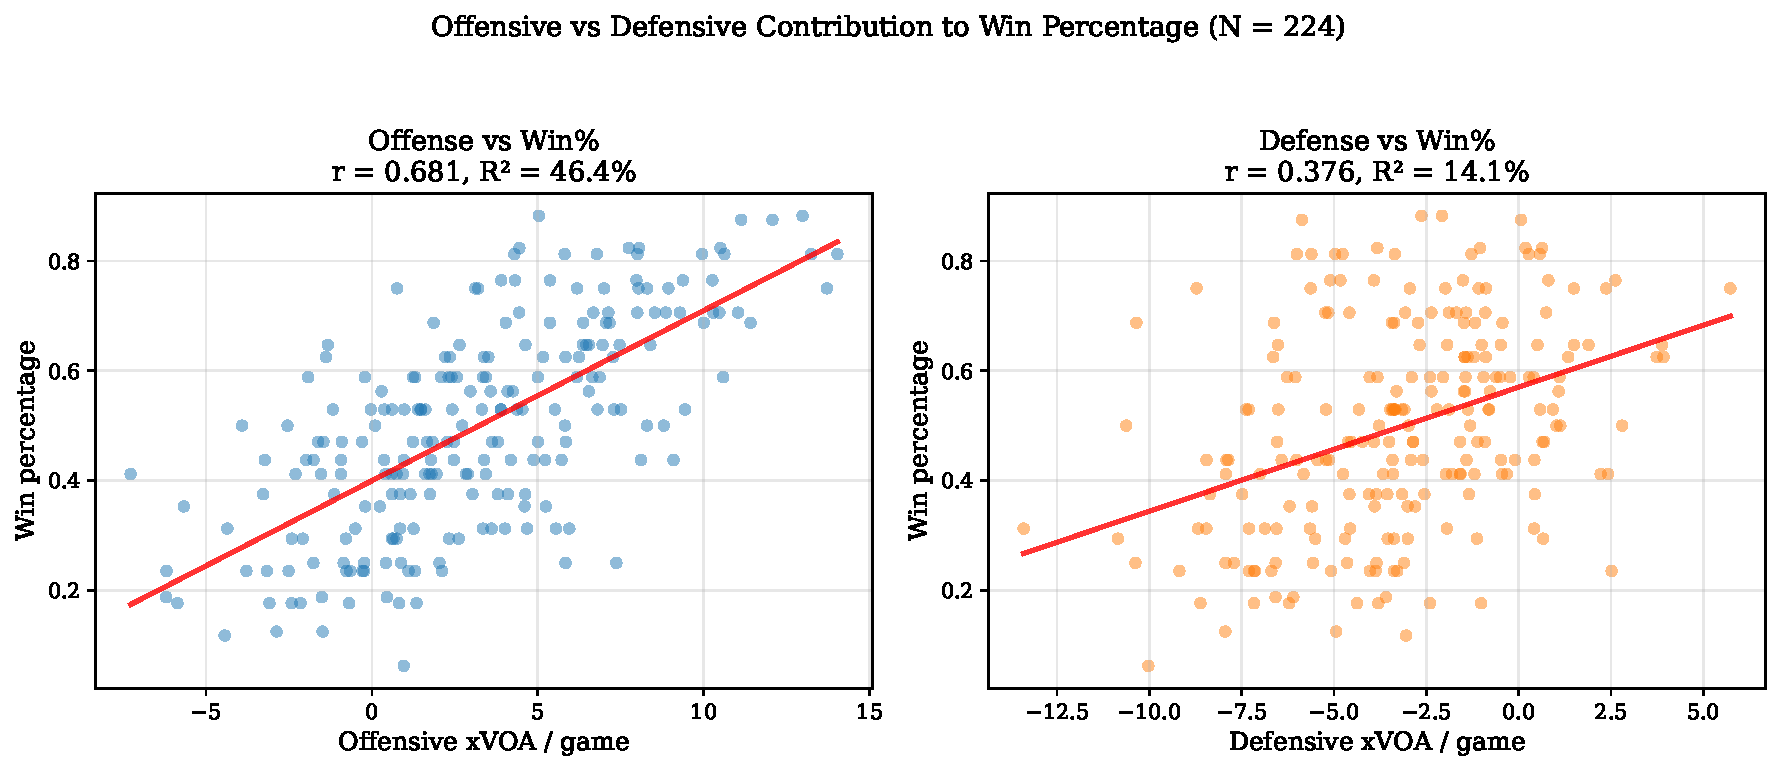
\includegraphics[width=\textwidth]{figures/fig3_xvoa_vs_winpct.pdf}
  \caption{Offensive (left) and defensive (right) \xvoa{}/game vs.\ win percentage ($n=256$ team-seasons, 2018--2025). The tighter clustering and steeper regression line for offense visualize the $R^2=44.5\%$ vs.\ $R^2=16.9\%$ split reported in \Cref{tab:components}.}
  \label{fig:xvoa-winpct}
\end{figure}

All five top teams derive the majority of their \gds{} from offense (Philadelphia is the only top-5 team with positive Def\_\xvoa{}), while the bottom five include teams with positive offensive \xvoa{} dragged down by catastrophic defensive underperformance (Carolina: $-10.852$ Def\_\xvoa{}/game) -- confirming that while offense dominates the top of the distribution, extreme defensive failure can still override positive offense at the bottom.

\begin{table}[htbp]
  \centering
  \caption{Top-5 and bottom-5 NFL teams by \gds{}/game in the 2024 regular season. Off and Def \xvoa{} reported per game.}
  \label{tab:top-bottom}
  \begin{tabular}{lrrrr}
    \toprule
    \textbf{Team} & \textbf{\gds{}/G} & \textbf{Off \xvoa{}/G} & \textbf{Def \xvoa{}/G} & \textbf{Win\%} \\
    \midrule
    \multicolumn{5}{l}{\textit{Top 5}} \\[2pt]
    DET & $+10.365$ & $+12.980$ & $-2.630$ & .882 \\
    PHI & $+8.384$  & $+7.740$  & $+0.639$ & .824 \\
    BAL & $+7.945$  & $+11.035$ & $-3.068$ & .706 \\
    TB  & $+6.729$  & $+10.586$ & $-3.822$ & .588 \\
    GB  & $+5.575$  & $+6.462$  & $-0.999$ & .647 \\[6pt]
    \multicolumn{5}{l}{\textit{Bottom 5}} \\[2pt]
    JAX & $-5.835$  & $+1.306$  & $-7.158$  & .235 \\
    NYG & $-6.158$  & $-2.417$  & $-3.799$  & .176 \\
    DAL & $-6.259$  & $+0.745$  & $-7.002$  & .412 \\
    CLE & $-6.700$  & $-5.861$  & $-1.012$  & .176 \\
    CAR & $-8.211$  & $+2.616$  & $-10.852$ & .294 \\
    \bottomrule
  \end{tabular}
\end{table}

An online supplement (\Cref{sec:supplement-pointer}) reports additional validation evidence not central to the paper's argument: a luck analysis quantifying win-loss divergence from \gds{}-implied expectations, a baseline comparison against raw point differential, per-season correlation stability across all eight years (range $r=0.818$ to $r=0.888$, with the new 2025 season at the high end), year-over-year rank stability, and split-half reliability (mean $\rho = 0.477$ across all eight seasons). Each confirms \gds{} behaves as a reliable measurement instrument; none changes the paper's conclusions, which is why they are summarized rather than reproduced here.

% ============================================================
% 4. ARCHETYPE CLASSIFICATION AND HYPOTHESIS-TESTING METHODS
% ============================================================
\section{Archetype Classification and Hypothesis-Testing Methods}
\label{sec:methods}

\subsection{Sample and Variables}
\label{sec:sample}

Using the \gds{} components defined in \Cref{sec:framework}, we classify each of the 256 team-seasons (32 teams $\times$ 8 seasons, 2018--2025) by the balance between its offensive and defensive contribution. The playoff subsample comprises 108 team-seasons; the Super Bowl winner subsample contains 8, one per season. All independent variables are computed from regular-season games only, ensuring temporal separation from the postseason outcomes used as dependent variables.

\Cref{tab:ivs,tab:dvs} define the variables. The key analytical variable, \texttt{offense\_share}, isolates the balance between offensive and defensive contribution independently of overall team quality:
\begin{equation}
  \label{eq:offense-share}
  \texttt{offense\_share} =
  \frac{\texttt{off\_xvoa\_per\_game}}
       {|\texttt{off\_xvoa\_per\_game}| + |\texttt{def\_xvoa\_per\_game}| + \varepsilon},
\end{equation}
where $\varepsilon = 0.01$ prevents division by zero for teams with negligible \xvoa{} in both channels and does not materially affect results at realistic per-game magnitudes (1--12 expected-point units). The variable ranges from $-1$ to $+1$ by construction; most team-seasons fall in $[-0.6, +0.6]$. We designate offense share, together with the $\pm0.3$ threshold split it produces, as the \textbf{primary specification} for the analyses that follow (Cohen's $d$, quadrant analysis); the quartile split and within-elite median split used elsewhere in the paper are explicit robustness checks against this primary specification, not parallel primary analyses -- \Cref{tab:operationalizations} in \Cref{sec:hypothesis-tests} cross-references every operationalization used anywhere in the paper against its sample definition, $N$, and result, so a reader need not track four coexisting definitions independently.

\begin{table}[htbp]
  \centering
  \caption{Independent variables. All computed at the team-season level from regular-season games only.}
  \label{tab:ivs}
  \begin{tabularx}{\textwidth}{llX}
    \toprule
    \textbf{Variable} & \textbf{Type} & \textbf{Definition} \\
    \midrule
    \texttt{offense\_share} & Continuous $[-1,+1]$ & Proportion of total absolute \xvoa{} attributable to offense (\Cref{eq:offense-share}). Positive = offense-dominant; negative = defense-dominant. \\[6pt]
    \texttt{gds\_per\_game} & Continuous & Mean \gds{}/game; overall team quality independent of offense/defense split. \\[6pt]
    \texttt{off\_xvoa\_per\_game} & Continuous & Mean offensive \xvoa{}/game. \\[6pt]
    \texttt{def\_xvoa\_per\_game} & Continuous & Mean defensive \xvoa{}/game. \\
    \bottomrule
  \end{tabularx}
\end{table}

\begin{table}[htbp]
  \centering
  \caption{Dependent variables.}
  \label{tab:dvs}
  \begin{tabularx}{\textwidth}{llX}
    \toprule
    \textbf{Variable} & \textbf{Type} & \textbf{Description} \\
    \midrule
    \texttt{win\_pct} & Continuous $[0,1]$ & Regular-season win fraction. \\[6pt]
    \texttt{playoff\_wins} & Ordinal $\{0,\dots,4\}$ & Postseason games won; 0 = missed playoffs or lost in round one. \\[6pt]
    \texttt{won\_super\_bowl} & Binary $\{0,1\}$ & Super Bowl victory indicator. \\
    \bottomrule
  \end{tabularx}
\end{table}

The three hypotheses (H1, H2, H3) are stated in \Cref{sec:introduction} and are not restated here.

\subsection{Statistical Procedures}
\label{sec:procedures}

Five procedures are employed, each motivated by the measurement level and distributional properties of the variables involved; the inferential conclusion rests on convergence across all five rather than any single $p$-value.

\textbf{Spearman rank correlation} between \texttt{offense\_share} and \texttt{playoff\_wins} across all 108 playoff team-seasons tests H1 and H3 -- appropriate because \texttt{playoff\_wins} is ordinal with a bounded 0--4 range and the relationship may be non-linear-monotonic. \textbf{Pearson correlation with $R^2$ decomposition} between each \xvoa{} component and win percentage across all 256 team-seasons directly compares variance explained. \textbf{Binary logistic regression} models Super Bowl victory as a function of offensive and defensive \xvoa{}/game:
\begin{equation}
  \label{eq:logistic}
  \log \frac{P(\texttt{won\_SB} = 1)}{P(\texttt{won\_SB} = 0)}
  = \beta_0 + \beta_1 \cdot \texttt{off\_xvoa/g} + \beta_2 \cdot \texttt{def\_xvoa/g}.
\end{equation}
With only 8 Super Bowl winners and 2 predictors, the events-per-variable ratio is 4.0, well below the recommended minimum of 10 \citep{hosmer2013logistic, peduzzi1996simulation}; we flag this once, here, and treat the model throughout the paper as a directional, exploratory supporting check rather than a source of primary evidence -- its coefficients are reported but do not appear as unqualified ``evidence'' in the hypothesis summary in \Cref{sec:hypothesis-tests}. \textbf{OLS regression} of \texttt{playoff\_wins} on both \xvoa{} components uses HC3 standard errors because the zero-inflated outcome produces heteroscedastic residuals; the Spearman correlation serves as a non-parametric check that does not impose linearity. \textbf{Cohen's $d$} is the standardized mean difference in playoff wins between offense-dominant (share $> +0.3$) and defense-dominant (share $< -0.3$) team-seasons, computed across the full sample (not restricted to playoff qualifiers) so that it captures both the selection effect (making the playoffs at all) and the advancement effect (winning once there), with conventional thresholds \citep{cohen1988statisticalpower} and a 95\% bootstrap confidence interval. A complementary \textbf{quartile analysis} partitions all 256 team-seasons into four equal groups by offense share as a non-parametric robustness check, reported alongside the primary specification in \Cref{tab:operationalizations}. No family-wise error correction is applied: the five procedures test the same substantive hypothesis from different angles, and the convergence-based inferential approach requires all five to agree rather than any one corrected test to pass, which is more conservative in practice.

\subsection{Robustness Design}
\label{sec:robustness-design}

Six checks address potential threats to validity. \textit{Opponent-strength control} re-estimates the OLS model with a leave-one-out opponent-quality covariate (mean \gds{}/game of all regular-season opponents faced, excluding the focal team's own contribution) to test whether the offensive advantage reflects schedule imbalance. \textit{Field-position mediation} \citep{baron1986moderator} quantifies the share of the offensive-\xvoa{}-to-wins association attributable to defense-generated starting field position, addressing the concern that offensive \xvoa{} is ``really'' measuring a downstream effect of defensive quality. \textit{Threshold sensitivity} varies the archetype threshold from $\pm0.20$ to $\pm0.40$. \textit{Time-window sensitivity} recomputes the offense-to-defense $R^2$ ratio across five overlapping windows spanning the full 2018--2025 range. \textit{Single-team exclusion} removes, in turn, Kansas City 2023 (the lowest offense share among champions, the most frequently cited counter-example before this paper's extension) and Seattle 2025 (the newest champion, to confirm the newest season alone is not driving the result). \textit{Era comparison} splits the sample at 2018--2020 versus 2021--2025; this comparison is explicitly exploratory given the small per-era subsamples and is intended to assess directional consistency, not to quantify a temporal trend.

% ============================================================
% 5. RESULTS -- VALIDATION & DESCRIPTIVE PATTERNS
% ============================================================
\section{Results: Descriptive Patterns}
\label{sec:descriptive}

\Cref{tab:quartile} partitions all 256 team-seasons into four equal groups by offense share; Q1 is the 64 most defense-dominant team-seasons, Q4 the 64 most offense-dominant.

\begin{table}[htbp]
  \centering
  \caption{Postseason outcomes by \texttt{offense\_share} quartile ($N=256$, 64 per quartile). Avg~PW includes non-qualifiers (playoff wins $=0$). Conf+ is conference championship or better (playoff wins $\geq 3$).}
  \label{tab:quartile}
  \begin{adjustbox}{max width=\textwidth}
  \begin{tabular}{lcrrrrr}
    \toprule
    \textbf{Quartile} & \textbf{N} & \textbf{Avg Share} & \textbf{Playoff\%} & \textbf{Avg PW} & \textbf{Conf+\%} & \textbf{SB Win\%} \\
    \midrule
    Q1 (Defense) & 64 & $-0.351$ & \phantom{0}9.4 & 0.016 & \phantom{0}0.0 & 0.0 \\
    Q2           & 64 & $+0.310$ & 15.6           & 0.047 & \phantom{0}0.0 & 0.0 \\
    Q3           & 64 & $+0.574$ & 56.3           & 0.516 & \phantom{0}3.1 & 3.1 \\
    Q4 (Offense) & 64 & $+0.817$ & 87.5           & 0.984 & 12.5           & 9.4 \\
    \bottomrule
  \end{tabular}
  \end{adjustbox}
\end{table}

\begin{figure}[htbp]
  \centering
  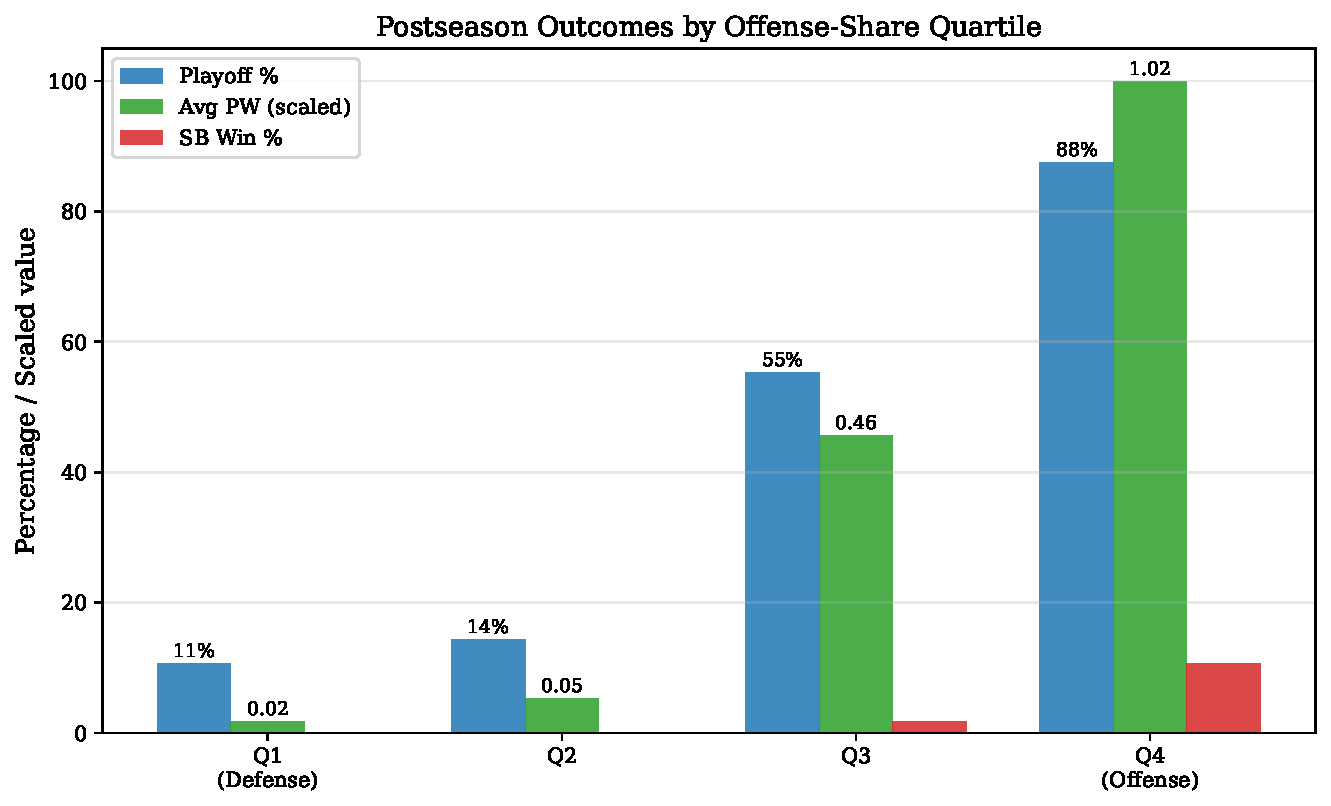
\includegraphics[width=0.85\textwidth]{figures/fig4_quartile_bars.pdf}
  \caption{Postseason outcomes by offense-share quartile. The monotonic gradient from Q1 (defense-dominant) to Q4 (offense-dominant) is visible across playoff qualification, average playoff wins, and Super Bowl victories.}
  \label{fig:quartile-bars}
\end{figure}

The gradient runs opposite to the defensive prediction: playoff appearance rises from 9.4\% (Q1) to 87.5\% (Q4), and mean playoff wins rise from 0.016 to 0.984, a roughly sixty-fold difference. Deep playoff success (conference championship or better) is essentially absent from the bottom half of the distribution -- 0.0\% in Q1 and Q2, the 128 most defense-dominant team-seasons in the dataset -- and is concentrated in Q3 and Q4, where all eight Super Bowl victories fall.

\Cref{tab:sb-participants} lists every team-season that won three or more playoff games in the study window, now including two 2025 entries: New England, who reached Super Bowl LX as a non-bye team with three playoff wins before losing (the same pattern as the 2021 Cincinnati Bengals in the table below), and Seattle, the 2025 Super Bowl champion. Every Super Bowl winner is unambiguously offense-dominant (share $+0.581$ to $+0.923$); five of the eight recorded \emph{negative} defensive \xvoa{}/game. Kansas City's 2022 title remains the clearest illustration: a defense at $-3.835$ \xvoa{}/game, well below league average, carried by an offense at $+10.498$. Seattle's 2025 title is a different profile worth noting explicitly, since it is the season this paper's extension was designed to test: Seattle's defensive \xvoa{} ($+3.104$/game) is the strongest of any champion in the sample, yet the team remains clearly offense-dominant (share $+0.650$) because its offense ($+5.782$/game) still exceeds its defense in absolute value -- a genuinely new data point that lands inside the pattern established by the other seven champions rather than breaking it. \textbf{No net-defense team (offense share $<0$) won more than one playoff game across eight seasons and 108 playoff team-seasons;} at the stricter defense-dominant threshold ($<-0.3$) used for formal hypothesis testing, zero of 32 such team-seasons won any playoff game.

\begin{table}[htbp]
  \centering
  \caption{Teams with $\geq 3$ playoff wins, 2018--2025. Off/G and Def/G are mean per-game \xvoa{}. Share is \texttt{offense\_share}. PW is playoff wins.}
  \label{tab:sb-participants}
  \begin{adjustbox}{max width=\textwidth}
  \begin{tabular}{llrrrrl}
    \toprule
    \textbf{Season} & \textbf{Team} & \textbf{Off/G} & \textbf{Def/G} & \textbf{Share} & \textbf{PW} & \textbf{SB} \\
    \midrule
    2018 & NE   & $+5.378$  & $-1.191$ & $+0.817$ & 3 & Win \\
    2019 & KC   & $+8.044$  & $-1.991$ & $+0.801$ & 3 & Win \\
    2020 & TB   & $+10.015$ & $-2.727$ & $+0.785$ & 4 & Win \\
    2021 & CIN  & $+6.649$  & $-1.456$ & $+0.819$ & 3 &  -- \\
    2021 & LA   & $+8.540$  & $-2.374$ & $+0.782$ & 4 & Win \\
    2022 & KC   & $+10.498$ & $-3.835$ & $+0.732$ & 3 & Win \\
    2023 & KC   & $+2.663$  & $+1.890$ & $+0.584$ & 4 & Win \\
    2024 & PHI  & $+7.749$  & $+0.635$ & $+0.923$ & 4 & Win \\
    2025 & NE   & $+8.013$  & $-1.599$ & $+0.833$ & 3 &  -- \\
    2025 & SEA  & $+5.782$  & $+3.104$ & $+0.650$ & 3 & Win \\
    \bottomrule
  \end{tabular}
  \end{adjustbox}
\end{table}

\begin{figure}[htbp]
  \centering
  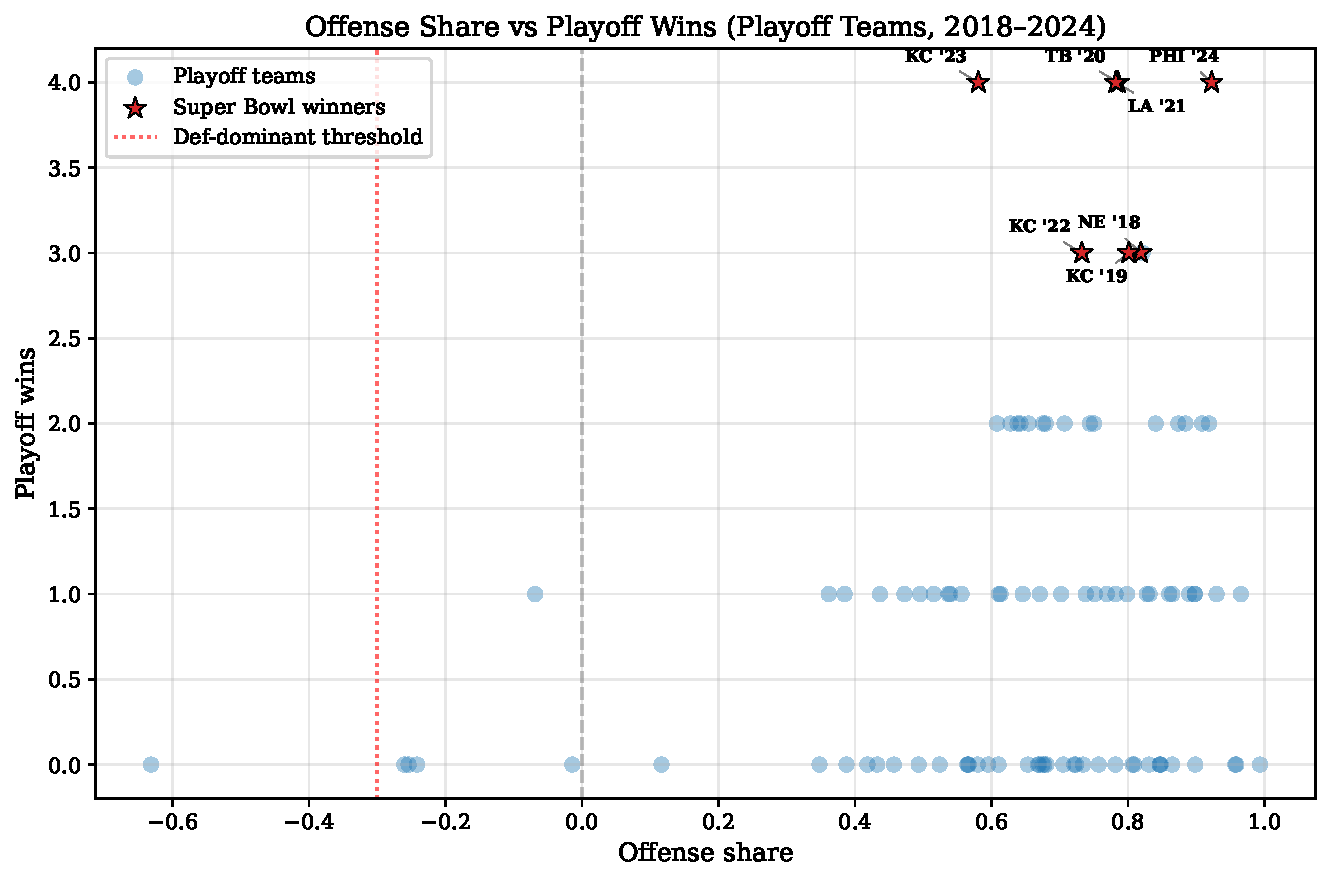
\includegraphics[width=0.85\textwidth]{figures/fig7_offense_share_pw.pdf}
  \caption{Offense share vs.\ playoff wins for all playoff team-seasons (2018--2025). Super Bowl winners (annotated) cluster in the offense-dominant region. No team below the defense-dominant threshold ($<-0.3$) won any playoff games.}
  \label{fig:offense-share-pw}
\end{figure}

% ============================================================
% 6. RESULTS -- HYPOTHESIS TESTS & ROBUSTNESS
% ============================================================
\section{Results: Hypothesis Tests and Robustness}
\label{sec:hypothesis-tests}

\subsection{The Five Tests}

\textbf{Spearman.} Across all 108 playoff team-seasons, $\rho = 0.208$ ($p = 0.0306$, 95\% bootstrap CI $[0.027, 0.377]$). The positive sign directly contradicts H3: higher offense share predicts \emph{more} playoff wins, not fewer. The coefficient is smaller than the 0.246 obtained from the 2018--2024 subsample alone, consistent with the ratio attenuation discussed in \Cref{sec:validation}, but remains significant and positive.

\textbf{Pearson / $R^2$.} As reported in \Cref{tab:components} (\Cref{sec:validation}), offensive \xvoa{} explains $R^2=44.5\%$ of win-percentage variance against $R^2=16.9\%$ for defensive \xvoa{} -- the 2.6:1 ratio that is this paper's central quantitative finding, here serving as the primary evidence against H3.

\textbf{Cohen's $d$.} $\bar{x}_{\text{off}} = 0.596$ playoff wins ($n=166$) vs.\ $\bar{x}_{\text{def}} = 0.000$ ($n=32$); $d = 0.669$ (95\% bootstrap CI $[0.580, 0.776]$) -- a medium-to-large effect directly contradicting H1, essentially unchanged from the 0.672 obtained on the 2018--2024 subsample alone despite the attenuation seen in the continuous measures. Not a single defense-dominant team-season won any playoff game; only one of the 32 (3.1\%) even qualified for the playoffs, and it was eliminated in the first round.

\textbf{Logistic regression.} \Cref{tab:logistic} reports the model. Both predictors are nominally significant, and the defensive coefficient is numerically larger (0.499 vs.\ 0.401), a gap that widened slightly relative to the 2018--2024-only estimate. As established in \Cref{sec:procedures}, the model's events-per-variable ratio (4.0) remains far below the recommended minimum, so this difference -- well within overlapping confidence intervals -- does not license a directional conclusion in either paper's version of the analysis. We report it as a supporting check consistent with the other four tests, not as independent evidence for H2; the primary basis for rejecting H2 is that all eight Super Bowl winners have positive offense share (\Cref{tab:sb-participants}), not the logistic coefficients.

\begin{table}[htbp]
  \centering
  \caption{Binary logistic regression predicting Super Bowl victory ($N=256$, 8 winners). Coefficients are log-odds; $p$-values are two-tailed Wald tests. Reported as a supporting check only -- see \Cref{sec:procedures} for the events-per-variable caveat.}
  \label{tab:logistic}
  \begin{tabular}{lrrr}
    \toprule
    \textbf{Predictor} & \textbf{Coef.} & \textbf{SE} & \textbf{$p$} \\
    \midrule
    Offensive \xvoa{}/game & $0.401$ & --- & $0.0019$ \\
    Defensive \xvoa{}/game & $0.499$ & --- & $0.0052$ \\
    \bottomrule
  \end{tabular}
\end{table}

\textbf{OLS.} $R^2 = 0.267$; $\hat{\beta}_{\text{off}} = 0.099$ ($p<0.0001$) vs.\ $\hat{\beta}_{\text{def}} = 0.071$ ($p<0.0001$) -- the offensive coefficient remains roughly 40\% larger, confirming the primacy of offensive quality for postseason advancement in a model that, unlike the logistic specification, is adequately powered.

\subsection{Consolidated Operationalizations}

Four distinct partitions of the sample appear across this paper: the continuous \texttt{offense\_share} variable (used directly in the Spearman and Pearson tests), the $\pm0.3$ threshold split (Cohen's $d$, quadrant analysis), the even quartile split (\Cref{tab:quartile}), and the within-elite median split used in the quadrant analysis below. \Cref{tab:operationalizations} cross-references all four against their sample definition, $N$, and result. The continuous variable and the $\pm0.3$ threshold split are the primary specification (\Cref{sec:sample}); the quartile and within-elite splits are robustness checks confirming the same pattern holds under alternative partitioning, not independent primary analyses.

\begin{table}[htbp]
  \centering
  \caption{Consolidated operationalizations of team archetype used in this paper. The continuous variable and $\pm0.3$ threshold (rows 1--2) are the primary specification; rows 3--4 are robustness checks.}
  \label{tab:operationalizations}
  \begin{adjustbox}{max width=\textwidth}
  \begin{tabular}{llrl}
    \toprule
    \textbf{Operationalization} & \textbf{Sample} & \textbf{$N$} & \textbf{Result} \\
    \midrule
    Continuous \texttt{offense\_share} (primary) & All playoff team-seasons & 108 & Spearman $\rho=0.208$, $p=0.031$ \\
    $\pm0.3$ threshold split (primary) & Off-dom.\ vs.\ def-dom. & 166 vs.\ 32 & Cohen's $d=0.669$ [0.580, 0.776] \\
    Even quartile split (robustness) & Full sample, 4 groups & 64 per group & Monotonic gradient, Q1$\to$Q4 (\Cref{tab:quartile}) \\
    Within-elite median split (robustness) & Top-quartile \gds{} only & 25 vs.\ 25 (of 64 elite) & Offense Only $>$ Defense Only on every metric (\Cref{tab:quadrant}) \\
    \bottomrule
  \end{tabular}
  \end{adjustbox}
\end{table}

\subsection{Quadrant Analysis of Elite Teams}
\label{sec:quadrant}

Restricting attention to top-quartile \gds{}/game team-seasons ($n=64$) and median-splitting within this elite subsample on offensive and defensive \xvoa{}/game separately yields four quadrants (\Cref{tab:quadrant}). The \textit{Offense Only} quadrant (above-median offense, below-median defense, $n=25$) recorded a higher Super Bowl rate (16.0\%), higher mean playoff wins (1.52), and higher conference-championship rate (20.0\%) than \textit{Defense Only} ($n=25$: 12.0\%, 1.08, 16.0\%) on every metric, though the gap is narrower than in the 2018--2024-only sample. Among elite teams, above-median offense remains associated with somewhat greater championship success than above-median defense on every measure, though this quadrant comparison should be read as directionally consistent with the paper's primary findings rather than as strong independent evidence in its own right, given the small per-quadrant samples ($n=25$ and $n=7$).

\begin{table}[htbp]
  \centering
  \caption{Quadrant analysis of elite team-seasons (top-quartile \gds{}/game, $n=64$), classified by within-elite medians for offensive and defensive \xvoa{}/game (off median $=7.610$, def median $=-1.465$).}
  \label{tab:quadrant}
  \begin{tabular}{lcrrrr}
    \toprule
    \textbf{Quadrant} & \textbf{N} & \textbf{Playoff\%} & \textbf{Avg PW} & \textbf{Conf+\%} & \textbf{SB Win\%} \\
    \midrule
    Elite Both      & \phantom{0}7 & \phantom{0}85.7 & 1.286 & 14.3 & 14.3 \\
    Offense Only    & 25           & \phantom{0}96.0 & 1.520 & 20.0 & 16.0 \\
    Defense Only    & 25           & \phantom{0}96.0 & 1.080 & 16.0 & 12.0 \\
    Neither         & \phantom{0}7 & \phantom{0}85.7 & 0.571 & \phantom{0}0.0 & \phantom{0}0.0 \\
    \bottomrule
  \end{tabular}
\end{table}

\begin{figure}[htbp]
  \centering
  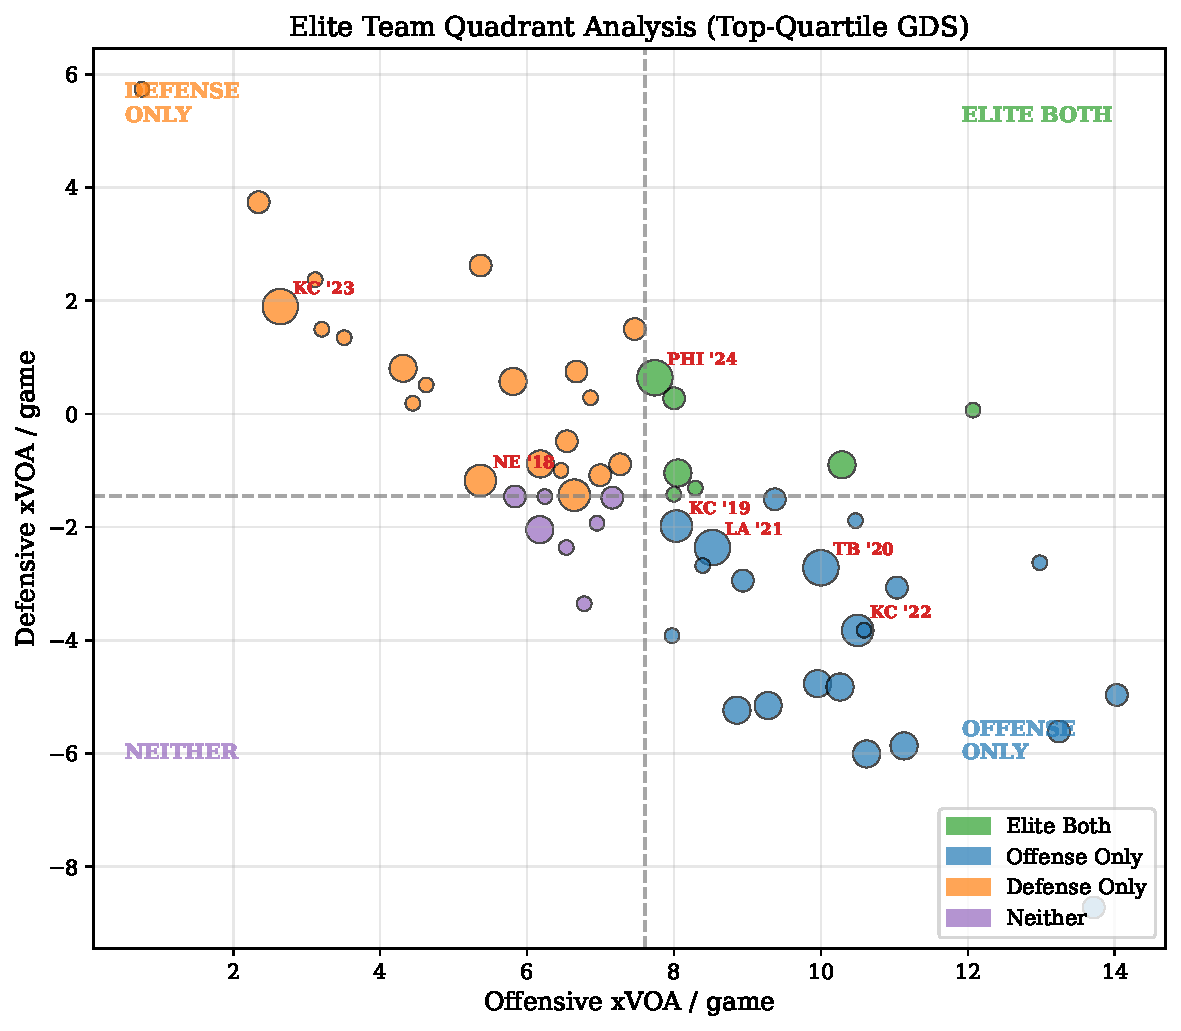
\includegraphics[width=0.8\textwidth]{figures/fig10_quadrant_diagram.pdf}
  \caption{Elite team quadrant analysis. Each point is a top-quartile \gds{} team-season, positioned by offensive (x-axis) and defensive (y-axis) \xvoa{}/game. Dashed lines indicate within-elite medians. Super Bowl winners are annotated.}
  \label{fig:quadrant}
\end{figure}

\subsection{Robustness Summary}
\label{sec:robustness-results}

\Cref{tab:robustness-summary} consolidates all six robustness checks, now including the additional single-team exclusion of Seattle 2025. Full per-check detail (opponent-strength control coefficients, the mediation decomposition, complete time-window and threshold sensitivity tables, and full era-comparison correlations) is reported in the online supplement (\Cref{sec:supplement-pointer}); the summary below is sufficient to establish that the offensive advantage is not an artifact of any single design choice, time window, or observation.

\begin{table}[htbp]
  \centering
  \caption{Robustness check summary. Full detail in the online supplement.}
  \label{tab:robustness-summary}
  \begin{adjustbox}{max width=\textwidth}
  \begin{tabular}{llX}
    \toprule
    \textbf{Check} & \textbf{Key statistic} & \textbf{Conclusion} \\
    \midrule
    Opponent-strength control & $\hat\beta_{\text{opp}} = -0.013$, $p=0.830$ & Offensive coefficient unchanged after controlling for schedule strength \\
    Field-position mediation & $8.0\%$ mediated & $92\%$ of the offense-wins association is independent of defense-generated field position \\
    Threshold sensitivity ($\pm0.20$ to $\pm0.40$) & Mean PW $= 0.000$ at every threshold ($n=26$--$42$) & Defense-dominant teams win zero playoff games regardless of boundary \\
    Time-window sensitivity (5 windows within 2018--2025) & Ratio range $2.5$:$1$ to $3.2$:$1$ & Offensive advantage holds in every window; never drops below $2.5$:$1$ \\
    Single-team exclusion (KC 2023; separately, SEA 2025) & Ratio $2.7$:$1$ either way; Spearman $\rho=0.221$ and $0.215$ respectively (both $p<0.05$) & No conclusion depends on the most-cited counter-example or on the newest season alone \\
    Era comparison (2018--20 vs.\ 2021--25) & Spearman positive in both eras (0.305, 0.163); neither individually significant & Directionally consistent; era subsamples too small for formal trend inference (see \Cref{sec:limitations}) \\
    \bottomrule
  \end{tabular}
  \end{adjustbox}
\end{table}

\subsection{Hypothesis Verdict}
\label{sec:verdict}

\Cref{tab:hypothesis-summary} consolidates the evidence. All three hypotheses are rejected, convergently, across five statistical procedures, two descriptive partitioning strategies, and six robustness checks. No procedure or partition produces evidence in the direction the defensive claim predicts, and the pattern is unchanged when the analysis is extended to include a season the underlying measurement framework had never seen.

\begin{table}[htbp]
  \centering
  \caption{Hypothesis testing summary. The logistic regression appears only as a supporting check for H2, consistent with its events-per-variable limitation (\Cref{sec:procedures}); the primary evidence for each hypothesis comes from adequately powered procedures.}
  \label{tab:hypothesis-summary}
  \small
  \begin{tabularx}{\textwidth}{l p{3.0cm} X l}
    \toprule
    \textbf{Hyp.} & \textbf{Claim} & \textbf{Primary evidence} & \textbf{Verdict} \\
    \midrule
    H1 & Defense-dominant teams win more playoff games
      & Cohen's $d=+0.669$ [0.580, 0.776] in opposite direction; off-dominant PW $=0.60$ vs.\ def-dominant PW $=0.00$; $0/32$ defense-dominant teams won any PW
      & \textbf{Rejected} \\[8pt]
    H2 & SB winners are defense-dominant
      & All 8 champions had positive offense share ($+0.581$ to $+0.923$); logistic model (supporting only, EPV $=4.0$) shows no directional signal favoring defense
      & \textbf{Rejected} \\[8pt]
    H3 & Def \xvoa{} has stronger association with PW
      & Spearman $\rho=+0.208$ ($p=0.031$); Pearson off $R^2=44.5\%$ vs.\ def $R^2=16.9\%$ ($2.6\times$); OLS $\beta_{\text{off}}=0.099>\beta_{\text{def}}=0.071$
      & \textbf{Rejected} \\
    \bottomrule
  \end{tabularx}
\end{table}

% ============================================================
% 7. DISCUSSION
% ============================================================
\section{Discussion}
\label{sec:discussion}

\subsection{Interpreting the Rejection}

The central empirical question receives an unambiguous answer, and it is not marginal or dependent on a particular procedure: it is consistent across five statistical tests, two descriptive partitioning strategies, six robustness checks, and both era subsamples, and it holds on the 2025 season specifically, which entered the analysis after every other component of the framework was already built. Among 32 defense-dominant team-seasons, zero won any playoff game, zero reached a conference championship, and zero appeared in a Super Bowl -- a null result against 108 total playoff team-seasons large enough that it cannot reasonably be attributed to chance.

\subsection{The Competent Defense Threshold}
\label{sec:threshold}

Rejecting the defensive hypothesis is not a claim that defense is irrelevant. Offensive quality is the primary engine of playoff qualification and advancement, while competent defense operates as a necessary but insufficient condition at the championship margin -- the distinction between being the \emph{driver} of success and being a \emph{filter} for the final stage. Five of eight champions recorded negative defensive \xvoa{}/game; Kansas City won the 2022 title with defensive \xvoa{} at $-3.835$/game, substantially below average, carried by an elite offense. Seattle's 2025 title illustrates the other end of the same threshold: its defense ($+3.104$/game) is the strongest among all eight champions, but the team still needed -- and had -- an offense that outweighed it ($+5.782$/game) to remain offense-dominant. A team with elite offense and below-average defense has won the Super Bowl in this sample; a team with elite defense and below-average offense has not. The threshold is asymmetric: the minimum offensive requirement for championship contention is substantially higher than the minimum defensive requirement.

\subsection{Structural Explanations}
\label{sec:structural}

Offensive production exhibits higher between-team variance than defensive production -- offensive schemes are more diverse, quarterback quality varies more across rosters than any defensive position, and the passing game creates more opportunity for between-team separation than the more constrained action space of defensive play; higher-variance predictors mechanically produce stronger correlations with outcomes. The post-2018 rule environment plausibly amplifies this further: expanded pass-interference and roughing-the-passer enforcement and restrictions on downfield contact \citep{pereira2018roughing, barnwell2019passingrevolution} constrain the tools available to even elite defensive units. We note, however, that the era-comparison evidence for this second mechanism is weaker in the extended sample than it appeared in the 2018--2024-only analysis: the offensive Pearson coefficient strengthens from 0.622 (2018--2020) to 0.701 (2021--2025), but the defensive coefficient also strengthens slightly (0.397 to 0.427) rather than declining, and neither era subsample's Spearman correlation reaches significance on its own (\Cref{tab:robustness-summary}). We report this honestly rather than retain a cleaner-sounding claim the updated data no longer supports; the rule-environment mechanism remains plausible on the strength of the cited rule changes themselves, but the era-correlation comparison should not be read as independent confirmation of it.

\subsection{Why the Myth Persists}
\label{sec:myth}

Availability bias combined with a denominator problem \citep{tversky1973availability} is the most plausible explanation for the belief's persistence despite weak empirical support: memorable defense-led championships (Seattle 2013, Denver 2015) are memorable precisely because they are statistically unusual, while the far more common failure of defense-dominant teams to reach the championship stage at all -- across eight seasons, most defense-dominant team-seasons never made the playoffs, and none won more than one game -- is invisible because absences generate no media narrative.

\subsection{Strategic Implications}
\label{sec:strategic}

Under the salary cap's zero-sum structure, the 2.6:1 $R^2$ ratio carries resource-allocation implications -- \emph{conditional on these associations at least partially reflecting causal mechanisms}, a qualification we state here, in the Abstract, and in the Introduction rather than only here. If marginal offensive investment yields higher expected returns than marginal defensive investment, a strategy allocating asymmetrically toward offense while avoiding catastrophic defensive weakness (the pattern occupied by five of eight champions) is not ``unbalanced'' in any meaningful sense; it is responding to the evidence \citep{mulholland2019optimizing}. This is an inference from correlational data, not a demonstration, and should be weighed alongside domain expertise and the limitations below rather than treated as a proven prescription.

\subsection{Limitations}
\label{sec:limitations}

First, the eight-season window (2018--2025) limits generalizability to this specific rule era; whether the offensive advantage is a structural truth about football or a rule-era artifact cannot be determined from these data alone. Second, \gds{} does not adjust for opponent quality at the drive level; the season-level opponent-strength control was null ($\hat\beta=-0.013$, $p=0.830$), providing reassurance but not a substitute for a principled drive-level adjustment. Third, the \xscore{} model conditions only on situational features, not personnel, so \gds{} cannot distinguish a team overperforming because of elite talent from one overperforming because of scheme or opponent weakness -- and elite quarterback quality in particular is a plausible confound, since elite quarterbacks simultaneously drive offense share and playoff success through channels this analysis cannot separate. Fourth, and most consequentially, the analysis documents statistical association, not causation: the finding that offensive \xvoa{} covaries more strongly with winning does not demonstrate that investing in offensive talent causes teams to win more games, and a specific concern is reverse causation through game state (teams with early leads shift to conservative play-calling), which score-differential conditioning mitigates but does not eliminate. Fifth, the logistic regression is substantially underpowered (EPV $=4.0$); it is treated throughout as a supporting check rather than primary evidence, and the primary evidential basis rests on the full-sample tests ($n=108$ and $n=256$). Sixth, the era subsamples are too small for formal inference on temporal trends, and, as \Cref{sec:structural} makes explicit, the era-comparison evidence for one of the two proposed structural mechanisms weakened once the 2025 season was added -- a reminder that exploratory subgroup comparisons of this kind should be weighted cautiously even when they point in a theoretically plausible direction. Seventh, \gds{}'s special-teams component is constructed from field-position deviation only and does not independently model special-teams scoring events, and the model's drive-start conditioning means intra-drive events are not independently evaluated.

% ============================================================
% 8. CONCLUSION
% ============================================================
\section{Conclusion}
\label{sec:conclusion}

We introduced \gds{}, the first fully transparent, reproducible NFL team-quality metric with explicit three-component decomposition, and validated it against actual game outcomes across eight seasons: 85.7\% game-winner accuracy and 74.3\% of season win-percentage variance explained ($r=0.862$, $n=256$ team-seasons) before using it for anything else. Applying the validated framework to the ``defense wins championships'' hypothesis, we find all three pre-specified directional hypotheses rejected, convergently, across five statistical procedures, two descriptive partitions, and six robustness checks: offensive \xvoa{} explains 2.6 times more win-percentage variance than defensive \xvoa{}, offense-dominant teams dramatically outperform defense-dominant teams in playoff advancement, and every Super Bowl champion in the study window -- including the 2025 champion, scored entirely out-of-sample relative to the underlying model -- was offense-dominant. The ``competent defense threshold'' framework provides a theoretical contribution beyond mere rejection: offensive excellence drives championship contention while defensive adequacy is a necessary but insufficient secondary condition.

Extending the analysis by one full season beyond the original working paper that developed this framework provided a genuine, if modest, stress test: the categorical finding (zero defense-dominant playoff success) proved exactly as strong on new data as on the original sample, while the continuous variance-explained ratio moved from 3.3:1 to a more conservative 2.6:1. We treat this attenuation as informative rather than as a result to minimize -- it is the behavior a real, non-overfit effect should show when tested on data it has not seen, and every robustness check in \Cref{sec:robustness-results} confirms the ratio stays comfortably above 2:1 regardless of window or specification. These findings remain correlational, and any resource-allocation implications are conditional on the associations partially reflecting causal mechanisms -- a qualification we have carried through the abstract, introduction, and discussion rather than confining to a caveat late in the paper. Extensions warranting investigation include a principled drive-level opponent adjustment, player-level \xvoa{} attribution connecting team-level findings to individual talent evaluation, positional decomposition of offensive value (rushing vs.\ passing), and salary-cap efficiency analysis directly quantifying whether the defensive heuristic has measurably distorted the talent market. The complete codebase, trained model, and data pipeline are publicly available for replication, critique, and extension.

% ============================================================
% ONLINE SUPPLEMENT
% ============================================================
\section*{Note on the Online Supplement}
\label{sec:supplement-pointer}

An online supplement, referenced at several points above, reports: the luck analysis (win-loss divergence from \gds{}-implied expectation), the point-differential baseline comparison, per-season correlation stability across all eight years, year-over-year rank stability, split-half reliability, and full per-check detail for the six robustness analyses summarized in \Cref{tab:robustness-summary}. None of this material changes the paper's conclusions; it is reported separately because it supports rather than drives the central argument.

% ============================================================
% DATA AND CODE AVAILABILITY
% ============================================================
\section*{Data and Code Availability}

All play-by-play data are publicly available via the \texttt{nflfastR} package \citep{carl2021nflfastr}. The complete analytical codebase -- including model training, GDS computation, archetype classification, statistical testing, and figure generation -- is available at \url{https://github.com/lasse5mecha/nfl-xscore-gds}.

% ============================================================
% CONFLICTS OF INTEREST
% ============================================================
\section*{Conflicts of Interest}

The author declares no conflicts of interest.

% ============================================================
% AI DISCLOSURE
% ============================================================
\section*{Statement on Use of Artificial Intelligence}

This paper was developed with the assistance of Claude (Anthropic), a large language model used as a coding and writing tool. All research design decisions, modeling choices, hypothesis operationalization, and interpretation of results are solely the author's intellectual contributions. AI-generated code was reviewed and validated by the author.

% ============================================================
% REFERENCES
% ============================================================
\printbibliography

\end{document}
